\subjectPresentation{2}{XAI for the USA Census}{color2}

\subjectDevelopment{Analyse Fairness on the USA Census}{
	\begin{itemize}
		\item Can we find bias in the ML models?
		\item If so, can we use XAI to identify where's the problem?
	\end{itemize}
	\vfill
	\centering
	We used the 'SEX' as the sensible variable.
}{color2}

\subjectDevelopment{Trained Models}{
\begin{itemize}
	\item \textbf{Logistic Regression}
	
    \item \textbf{XGBoost} (eXtreme Gradient Boosting)
	
	\item \textbf{Hist Gradient Boosting} (Skrub's Scikit-learn implementation)
	
	\item \textbf{Simple Neural Network}
\end{itemize}
}{color2}

\subjectDevelopment{Fairness Metrics}{
\begin{itemize}
	\item \textbf{Accuracy}: The proportion of correct predictions (both true positives and true negatives) among all predictions.

	\item \textbf{Disparate Impact (DI)}: Measures the ratio between the \textbf{proportion of positive outcomes for the protected group (women) versus the privileged group (men)}. Values close to 1 indicate fairness, while values below 1 suggest bias against the protected group.

	\item \textbf{Equality of Odds}: Examines whether both groups have equal true positive rates and equal false positive rates. Values closer to 1 indicate better fairness.

	\item \textbf{Sufficiency}: Assesses whether the probability of the true outcome is the same across groups given the predicted outcome. Values closer to 1 indicate better fairness.
\end{itemize}
}{color2}

\subjectDevelopment{Performance and Fairness metrics}{
\begin{table}[h]
\centering
\caption{Model Performance Comparison Across States (Accuracy and Fairness Metrics)}
\label{tab:folktables-results}
\resizebox{\textwidth}{!}
{
\begin{tabular}{llcccccc}
\toprule
\textbf{Model} & \textbf{Training} & \textbf{Testing} & \textbf{Accuracy} & \textbf{Disparate Impact} & \textbf{Equality of Odds} & \textbf{Sufficiency} \\
\midrule
\rowcolor{gray!10}
\multirow{6}{*}{Logistic Regression} 
& \multirow{2}{*}{CA} & CA & 0.56 & 0.67 & 0.84 & 0.95 \\
& & USA & 0.52 & 0.66 & 0.88 & 0.86 \\
\cmidrule(lr){2-7}
& \multirow{2}{*}{TX} & TX & 0.52 & 0.46 & 0.65 & 0.90 \\
& & USA & 0.51 & 0.46 & 0.67 & 0.95 \\
\cmidrule(lr){2-7}
& \multirow{2}{*}{NY} & NY & 0.51 & 0.66 & 0.82 & 0.93 \\
& & USA & 0.52 & 0.64 & 0.86 & 0.88 \\
\midrule

\rowcolor{gray!10}
\multirow{6}{*}{XGBoost} 
& \multirow{2}{*}{CA} & CA & 0.64 & 0.72 & 0.91 & 0.96 \\
& & USA & 0.58 & 0.67 & 0.92 & 0.90 \\
\cmidrule(lr){2-7}
& \multirow{2}{*}{TX} & TX & 0.60 & 0.58 & 0.83 & 0.93 \\
& & USA & 0.58 & 0.58 & 0.85 & 0.95 \\
\cmidrule(lr){2-7}
& \multirow{2}{*}{NY} & NY & 0.61 & 0.75 & 0.92 & 0.96 \\
& & USA & 0.57 & 0.67 & 0.92 & 0.90 \\
\midrule

\rowcolor{gray!10}
\multirow{6}{*}{HistGradientBoosting} 
& \multirow{2}{*}{CA} & CA & 0.63 & 0.71 & 0.90 & 0.94 \\
& & USA & 0.58 & 0.67 & 0.92 & 0.90 \\
\cmidrule(lr){2-7}
& \multirow{2}{*}{TX} & TX & 0.61 & 0.54 & 0.78 & 0.96 \\
& & USA & 0.58 & 0.56 & 0.83 & 0.97 \\
\cmidrule(lr){2-7}
& \multirow{2}{*}{NY} & NY & 0.60 & 0.68 & 0.89 & 0.97 \\
& & USA & 0.58 & 0.64 & 0.90 & 0.91 \\
\midrule

\rowcolor{gray!10}
\multirow{6}{*}{Neural Network} 
& \multirow{2}{*}{CA} & CA & 0.52 & 0.88 & 1.03 & 0.85 \\
& & USA & 0.46 & 0.65 & 0.86 & 0.86 \\
\cmidrule(lr){2-7}
& \multirow{2}{*}{TX} & TX & 0.50 & 0.61 & 0.87 & 0.94 \\
& & USA & 0.49 & 0.77 & 0.96 & 0.81 \\
\cmidrule(lr){2-7}
& \multirow{2}{*}{NY} & NY & 0.51 & 0.76 & 0.93 & 0.92 \\
& & USA & 0.48 & 0.66 & 0.88 & 0.87 \\
\bottomrule
\end{tabular}%
}
\end{table}
}{color2}

\subjectDevelopment{Model Performance}{
\begin{figure}[h]
    \centering
	\vspace{-0.2cm}
	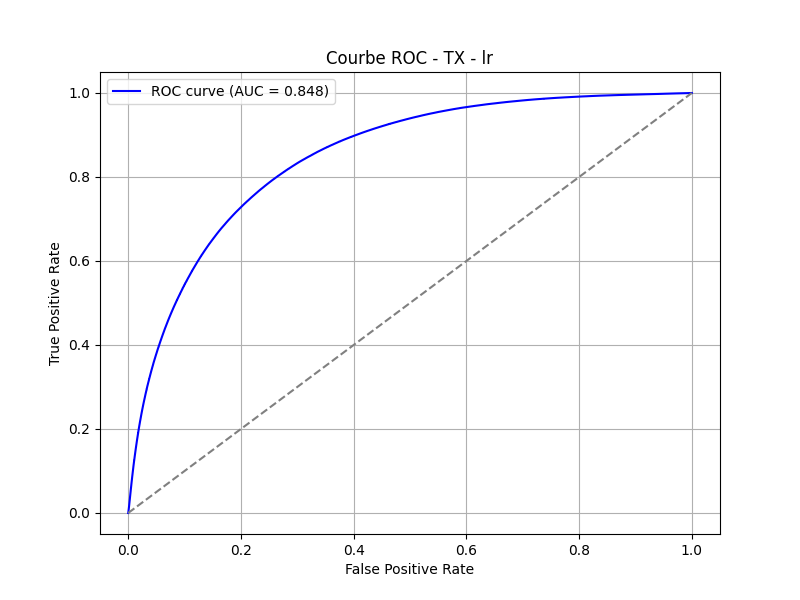
\includegraphics[width=0.45\textwidth]{Images/curve_roc_folktables/roc_curve_TX_lr.png}
	\hfill
	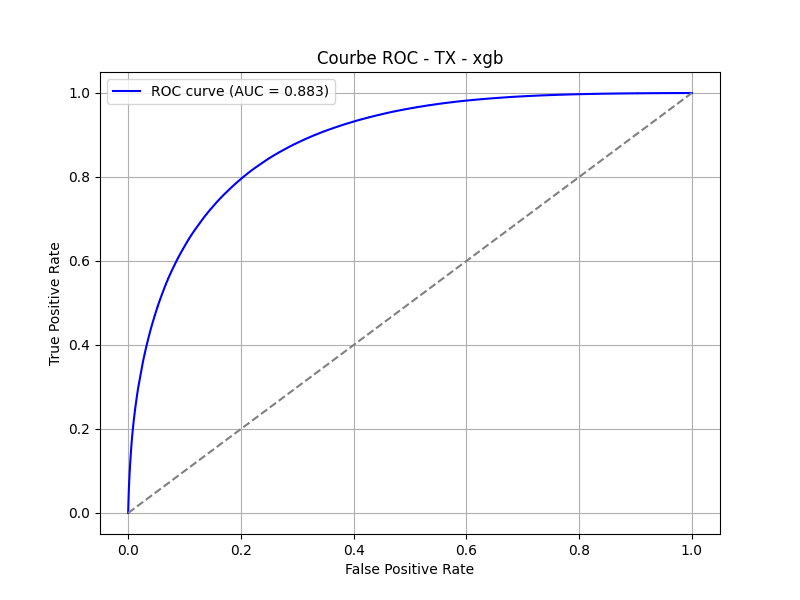
\includegraphics[width=0.45\textwidth]{Images/curve_roc_folktables/roc_curve_TX_xgb.png}
    \hfill
	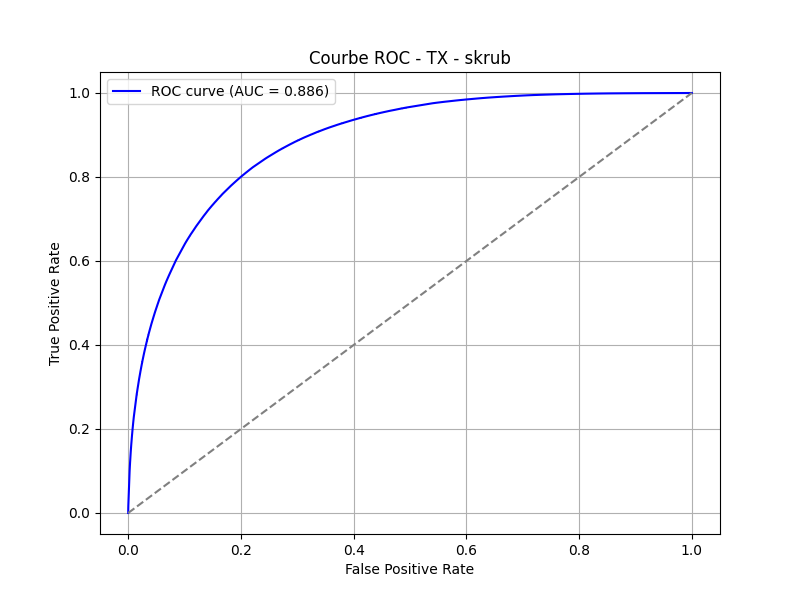
\includegraphics[width=0.45\textwidth]{Images/curve_roc_folktables/roc_curve_TX_skrub.png}
	\hfill
	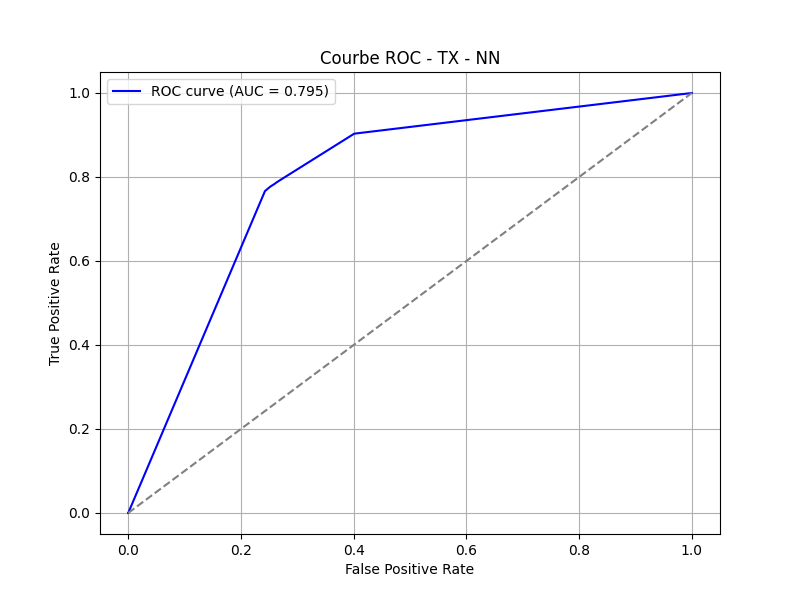
\includegraphics[width=0.45\textwidth]{Images/curve_roc_folktables/roc_curve_TX_NN.png}
    \caption{Comparison of the models trained on the sub dataset of the Texas state}
    \label{fig:roc_tx}
\end{figure}
}{color2}

\subjectDevelopment{Applying XAI}{
\begin{itemize}
	\item We will refer to a \textbf{gendered anchor} when the generated Anchors explanation contains 'SEX' in its list of features, which is the sensitive variable we are analysing.
	\item  In a similar way, we will refer to \textbf{gendered SHAP values} when the generated SHAP explanation contains 'SEX' at the top of the feature ranking.
\end{itemize}
}{color2}

\subjectDevelopment{Distribution of Gendered Anchors (Anchors vs SHAP)}{
\begin{figure}[h]
    \centering
	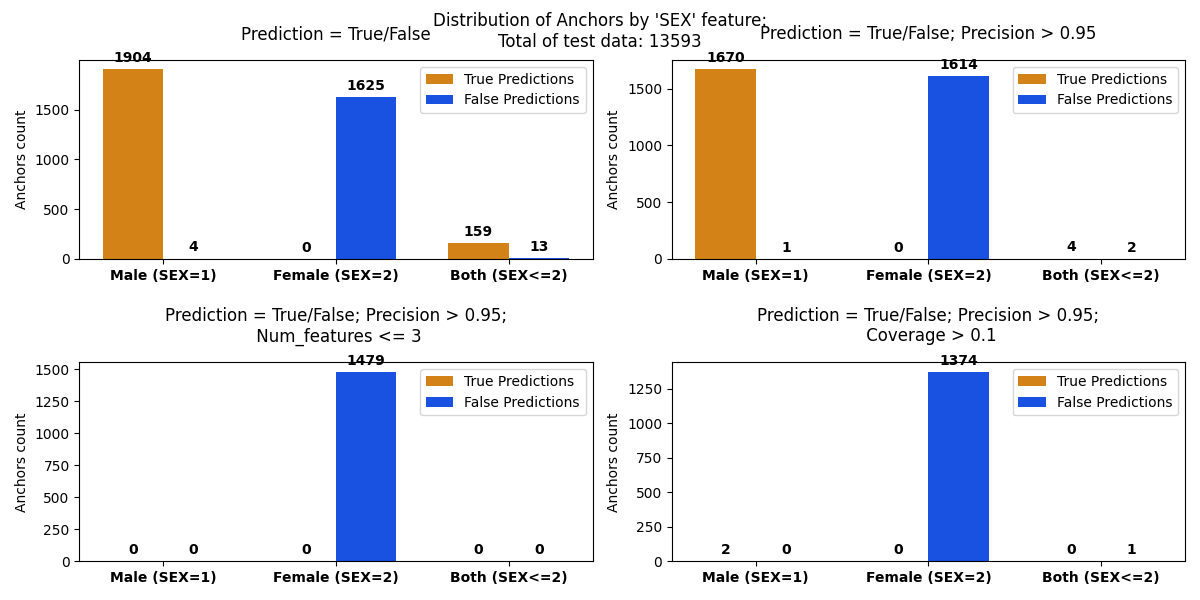
\includegraphics[width=\textwidth]{Images/folktables/distr_skrub_tx_anchors.png}
\end{figure}
}{color2}

\subjectDevelopment{Distribution of Gendered SHAP values}{
\begin{figure}[h]
    \centering
	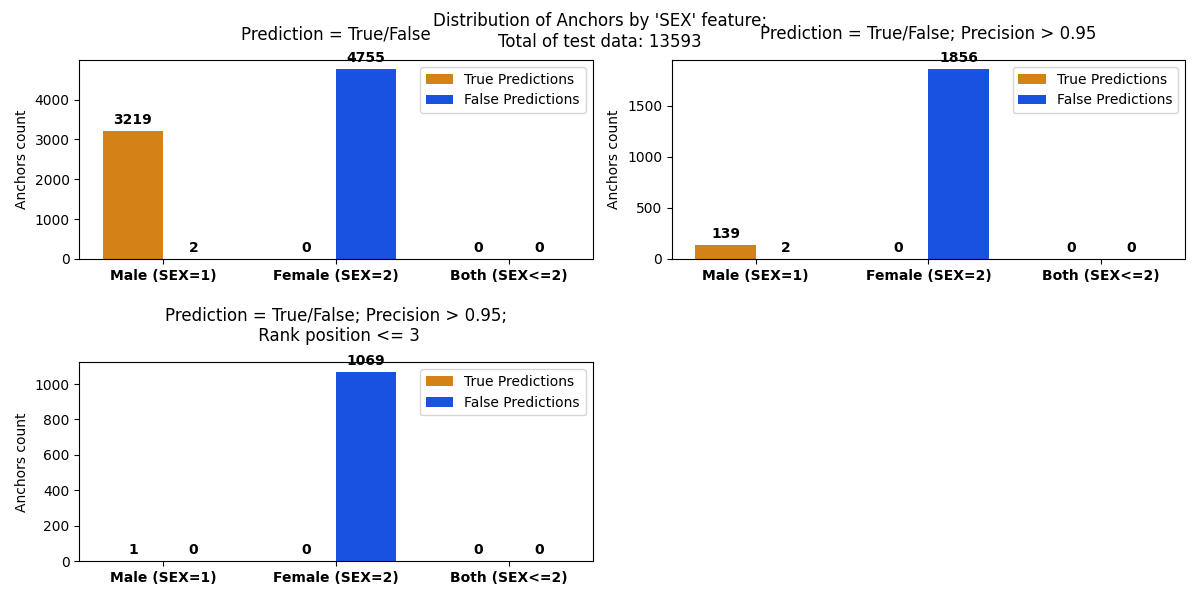
\includegraphics[width=\textwidth]{Images/folktables/distr_skrub_tx_shap.png}
\end{figure}
}{color2}

\subjectDevelopment{What does it mean?}{
	It was interesting to see how many explanations contained gendered explanations, meaning that the technique identified that feature as decisive for the prediction. 
\begin{itemize}
	\item With Anchors this implies that if the value of 'SEX' changes, the prediction changes too.
	\item We can also notice that the gendered explanations are divided mainly between \textbf{women with a false model prediction}, low income, and \textbf{men with a true prediction}, high income.
	\item \textbf{This reaffirms what the DI metric was showing:} this imbalance in the proportion of True predictions for the protected group versus the privileged group.
\end{itemize}
}{color2}

\subjectDevelopment{What can we do to go further in the investigation?}{
Analyse the profile of the test dataset to see how the Anchors and SHAP explanations are \textbf{organized across different groups of people}. To understand better the demographic problem in our study case.
}{color2}
